Now that we have presented the coordination facts for LM, we are now in a
position to use them in the SSSP program presented before.  The coordinated
version of the SSSP~(Fig.~\ref{code:shortest_path_program_coord}) uses the
coordination fact \texttt{set-priority} (line~\ref{line:coord:sssp_set}) and a global program directive
to order priorities in ascending order (line~\ref{line:coord:sssp_asc}).

When run with one thread, the algorithm behaves like Dijkstra's shortest path
algorithm~\cite{Dijkstra}. When using multiple threads, each thread will pick
the shortest distance from their subset of nodes.  While this does not yield the
optimal program with relation to 1 thread, it allows for parallel execution and
locally avoids unnecessary work. The result scales well and it is close to
Dijkstra's algorithm.

\begin{figure}[ht]
\begin{Verbatim}[numbers=left,commandchars=\\\{\},fontsize=\scriptsize]
type route edge(node, node, int).
type linear shortest(node, int, list int).
type linear relax(node, int, list int).

\underline{priority @order asc}.\label{line:coord:sssp_asc}

shortest(A, +00, []).
relax(@1, 0, [@1]).

shortest(A, D1, P1), D1 > D2, relax(A, D2, P2)
   -o shortest(A, D2, P2),
      \{B, W | !edge(A, B, W) |
         relax(B, D2 + W, P2 ++ [B]),
         \underline{set-priority(B, float(D2 + W))}\}.\label{line:coord:sssp_set}

shortest(A, D1, P1), D1 <= D2, relax(A, D2, P2)
   -o shortest(A, D1, P1).
\end{Verbatim}
   \caption{Shortest Path Program coordinated with \texttt{set-priority}.}
   \label{code:shortest_path_program_coord}
\end{figure}

%%% show new steps
Figure~\ref{fig:coordination:new_sssp} presents the 4 steps of computation for
the new SSSP program when executing with 1 thread. In every step a new shortest
path is computed at a different node, starting from the shorter paths up to
the longer paths. This is exactly the same behaviour as the Dijkstra's
algorithm.

\begin{figure}
\begin{center}
   \begin{subfigure}[b]{0.4\textwidth}
      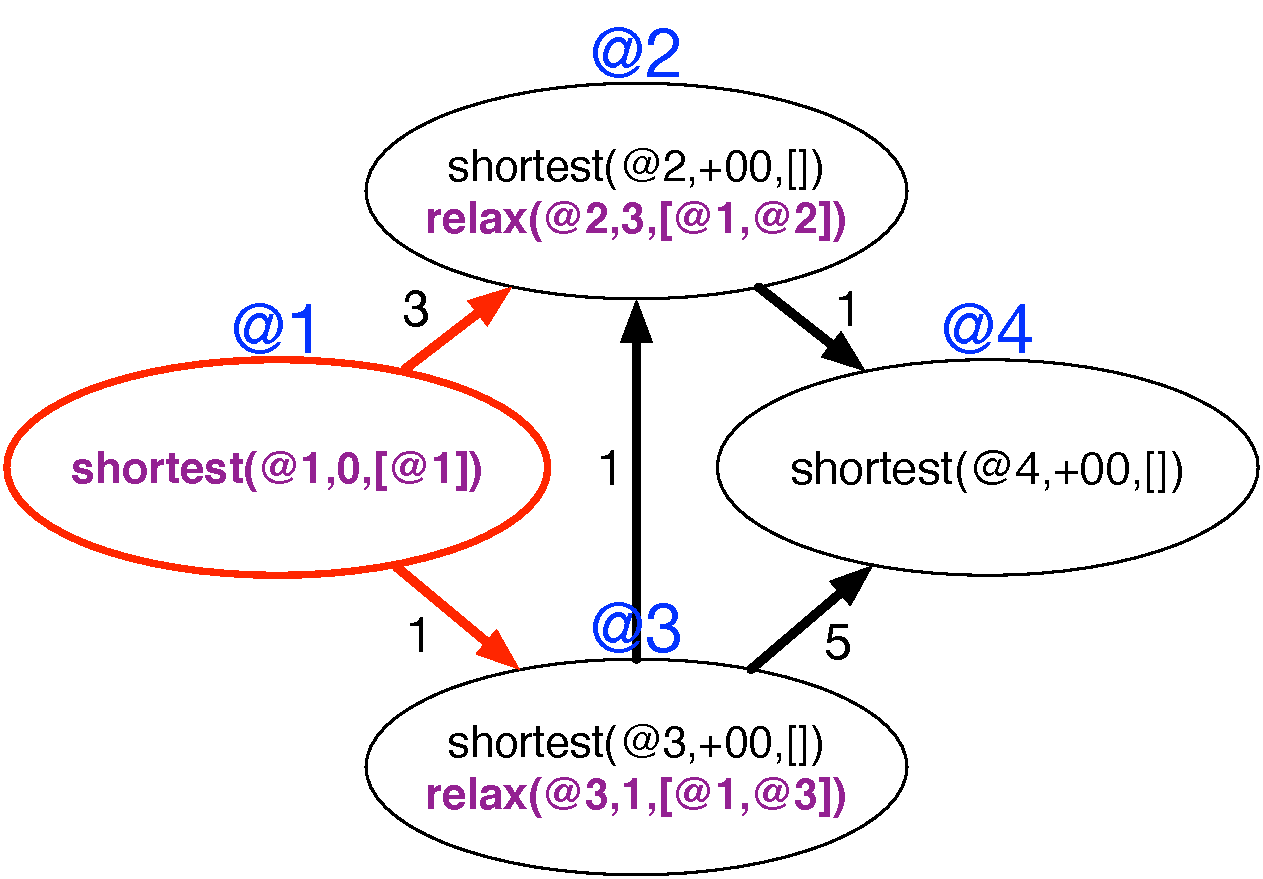
\includegraphics[width=\textwidth]{figures/sssp/coord1}
      \caption{}
   \end{subfigure}
   \begin{subfigure}[b]{0.4\textwidth}
      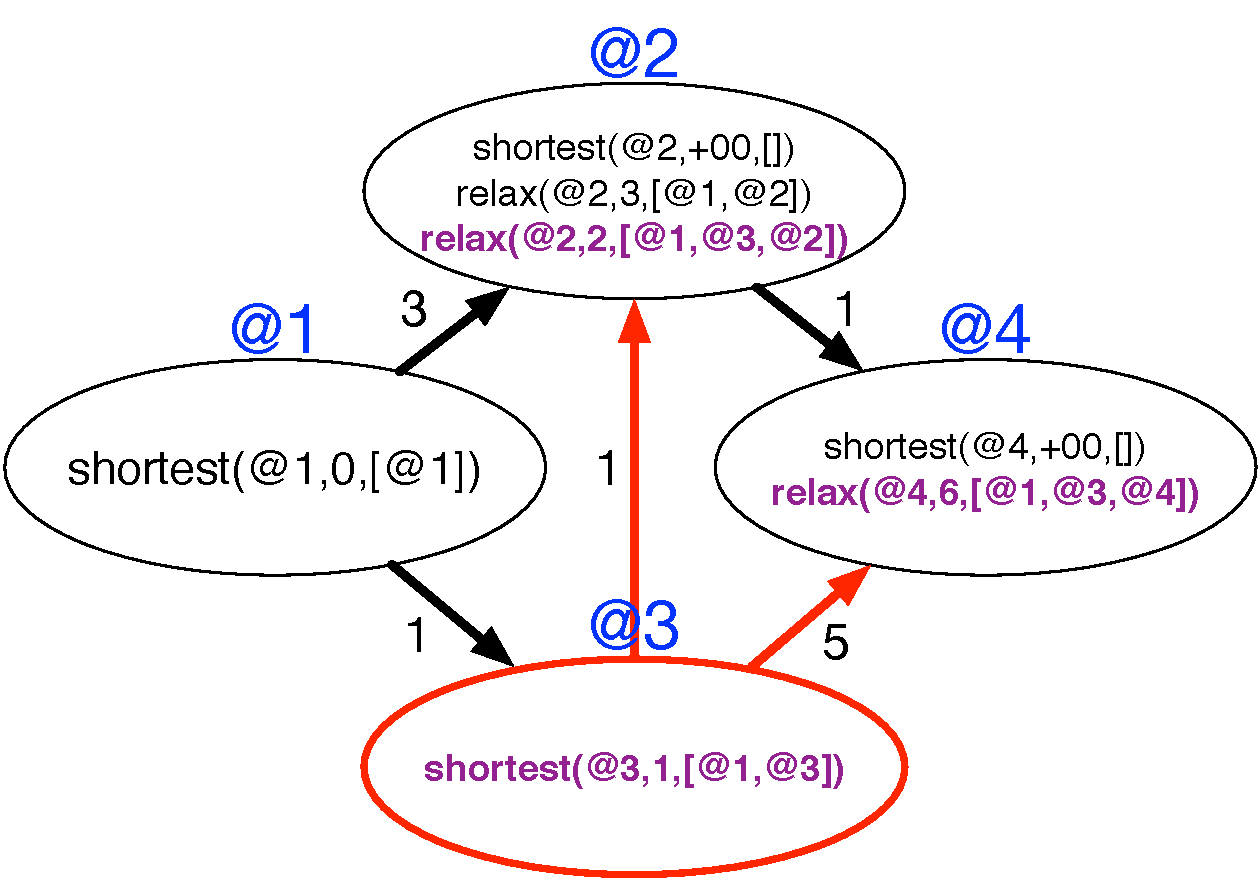
\includegraphics[width=\textwidth]{figures/sssp/coord2}
      \caption{}
   \end{subfigure}
   \begin{subfigure}[b]{0.4\textwidth}
      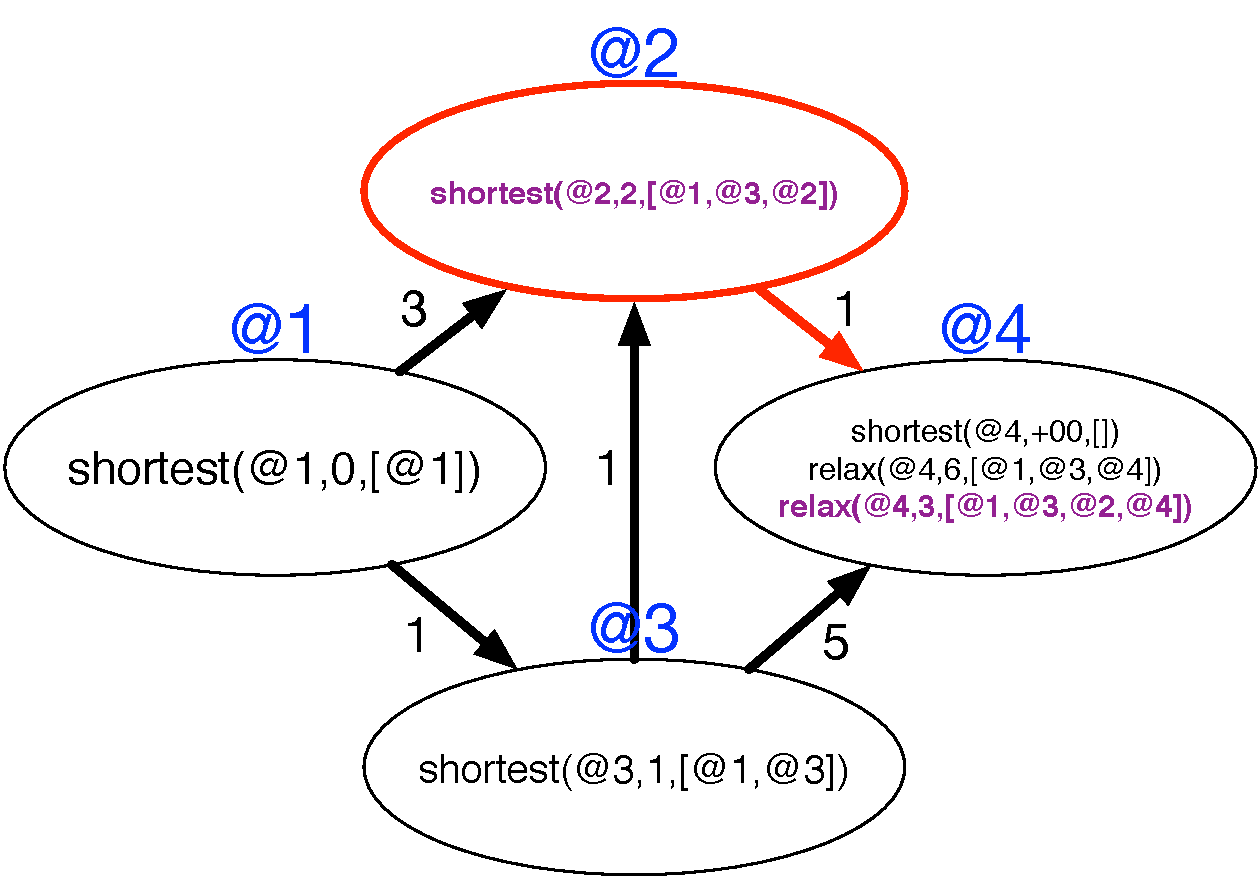
\includegraphics[width=\textwidth]{figures/sssp/coord3}
      \caption{}
   \end{subfigure}
   \begin{subfigure}[b]{0.4\textwidth}
      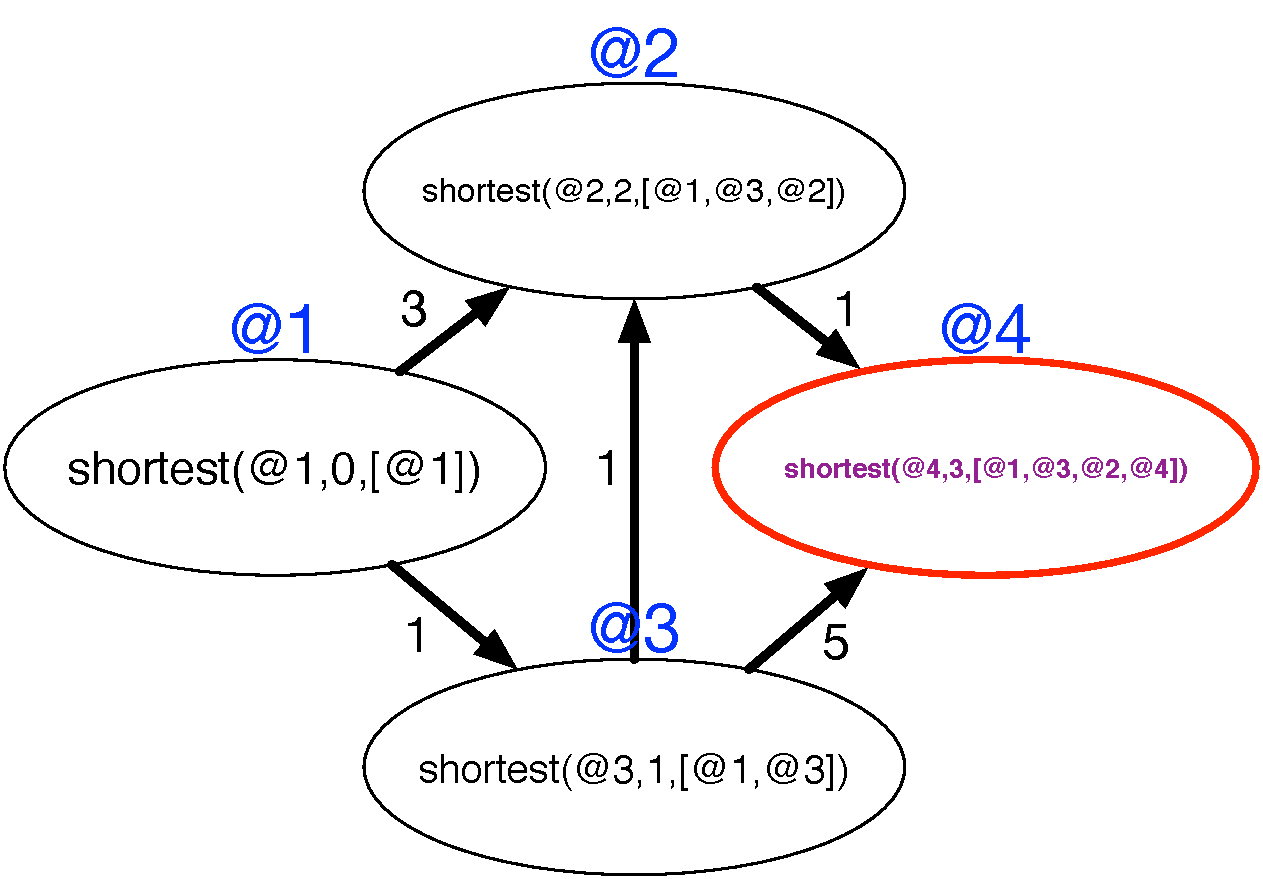
\includegraphics[width=\textwidth]{figures/sssp/coord4}
      \caption{}
   \end{subfigure}
\end{center}
\caption{Graphical representation of the new SSSP program. (a) represents the
   program after propagating initial distance at node \texttt{@1}, followed by
   (b) where the first rule is applied in node \texttt{@3}. (c)
   represents the result after retracting all the \texttt{relax} facts at node
   \texttt{@2} and (d) is the final state of the program where all the shortest paths
   have been computed.}
\label{fig:coordination:new_sssp}
\end{figure}

\subsection{Proof Of Correctness}

The most interesting property of the SSSP program presented in
Fig.~\ref{code:shortest_path_program_coord} is that it remains provably correct,
although it applies rules using a smarter ordering and the code remains
declarative. We now show the complete proof of correctness.

\begin{invariant}[Distance]

\texttt{relax(A, D, P)} represents a valid distance \texttt{D} and a valid path
\texttt{P} from node \texttt{@1} to node \texttt{A}. If the shortest distance to
\texttt{@1} is $D'$, then $D >= D'$.

\texttt{shortest(A, D, P)} represents a valid distance \texttt{D} and a valid
path \texttt{P} from node \texttt{@1} to node \texttt{A}. If the shortest
distance to \texttt{@1} is $D'$, then $D >= D'$. The \texttt{shortest} fact may
also represent an invalid distance if \texttt{D = +00}, where \texttt{P = []}.

\end{invariant}

\begin{proof}
By mutual induction. All the initial facts are valid and rule 1 and 2 validate the
invariant using the inductive hypothesis.
\end{proof}

\begin{lemma}[Relaxation]
Every new improved distance will be propagated to the neighbor nodes exactly once.
\end{lemma}
\begin{proof}
By rule 1, we know that when the distance is relaxed, we keep the new shorter
distance and propagate the distances. Every new distance that is longer will be
ignored by rule 2.
\end{proof}

\begin{theorem}[Correctness]

   Assume a graph $G = (V, E)$ where $W_{e \in E) >= 0}$ (positive weights).
   Consider that there is a set of nodes $S \in V$ where the shortest distances
   has been computed and a set $U \in V$ where it has not yet been reached.
   Sets are $S$ and $U$ are disjunct. At any given point, $\Sigma$ is the sum of
   all current shortest distances. For the distance \texttt{+00} we assign the
   value $\Sigma' + 1$, where $\Sigma'$ is the sum of the true shortest
   distances of nodes reachable from \texttt{@1}.  Every rule inference will
   either:

   \begin{itemize}
      \item Maintain the size of $S$ and reduce the total number of facts in
         the database.
      \item Increase the size of $S$, reduce $\Sigma$ and potentially increase the number of
         facts in the database.
      \item Maintain the size of $S$, decrease $\Sigma$
         and potentially increase the number of facts in the database.
   \end{itemize}

   Eventually, set $S = V$ and every \texttt{shortest(A, D, P)} will represent
   the shortest distance from \texttt{A} to \texttt{@1} and \texttt{P} is its
   corresponding path.
\end{theorem}

\begin{proof}
   By nested induction on $\Sigma$ and on the number of facts in the database.

   In the base case, we have \texttt{relax(@1, 0, [@1])} that will give us
   the shortest distance for node \texttt{@1}, therefore $S = \{@1\}$ and
   $\Sigma$ is reduced.

   In the inductive case, we have a set $S'$ where the shortest distance was
   reached and \texttt{relax} distances may have been propagated (Relaxation
   Lemma).

   Now consider the two rules of the program:

   \begin{itemize}

      \item Rule 1 will only apply at nodes in $U$. If the shortest
         \texttt{relax} is selected, then the node is added to $S$, otherwise it
         stays in $U$ but improves the shortest path, reduces $\Sigma$ and
         \texttt{relax} facts are generated (Relaxation Lemma).

      \item Rule 2 is applied in either nodes of $S$ or $U$. For both sets, the rule
         retracts the \texttt{relax} fact.

   \end{itemize}

   The case where rule 1 derives the true shortest distance happens when the
   node that minimizes $\argmin_t d(s \in S) + w(s, t)$ is selected, where
   $d(x)$ is the distance to the node \texttt{@1} and $w(a, b)$ the weight of
   the edge between $a$ and $b$. Using \texttt{set-priority} increases the
   probability of that node being selected, but it does not matter since
   the program always makes progress and the shortest distances will be
   eventually computed.
\end{proof}
